\chapter{Specifikacija programske potpore}
		
	\section{Funkcionalni zahtjevi}
			

			

				

			
			
			\noindent \textbf{Dionici:}
			
			\begin{packed_enum}
				
				\item Administrator
				\item Moderator			
				\item Korisnici aplikacije
					\begin{packed_enum}
						
						\item  Pregledavač
						\item  Običan korisnik
						\item  Premium korisnik
					
					\end{packed_enum}
				\item Razvojni tim	
				
			\end{packed_enum}
			
			\noindent \textbf{Aktori i njihovi funkcionalni zahtjevi:}
			
			
			\begin{packed_enum}
				\item  \underbar{Pregledavač/ neprijavljen korisnik (inicijator) može:}
				
				\begin{packed_enum}
					
					\item 	Otvoriti stranicu za prijavu
					\item 	Otvoriti stranicu za registraciju
					
					
				\end{packed_enum}
			
				\item  \underbar{Običan korisnik (inicijator) može:}
				
				\begin{packed_enum}
					
					\item Dodati obveze
					\item Dodati javne i privatne događaje te ih ocjenjivati
					\item Prijavljivati se na događaje
					\item Generirati svoj QR kod
					\item Preko QR koda dodati prijatelje
					\item Preko nadimka dodati, blokirati i ukloniti prijatelje
					\item Promjena nadimka profila
					
				\end{packed_enum}
			
				\item  \underbar{Premium korisnik (inicijator) može:}
				
				\begin{packed_enum}
					
					\item Promovirati vlastiti događaj
			
					
				\end{packed_enum}
			
				\item  \underbar{Moderator (inicijator) može:}
				
				\begin{packed_enum}
					
					\item Suspendirati korisnika
					\item Uređivati oznake javnih događaja
					\item Brisanje događaje
					
				\end{packed_enum}
			
				\item  \underbar{Administrator (inicijator) može:}
				
				\begin{packed_enum}
					
					\item Promovirati korisnika u moderatora
					\item Brisati korisničke račune
					
				\end{packed_enum}
			
				\item  \underbar{Baza podataka (sudionik):}
				
				\begin{packed_enum}
					
					\item Pohranjuje sve podatke o korisnicima i njihovim ovlastima
					\item Pohranjuje sve podatke o događajima i njihovim karakteristikama
					
				\end{packed_enum}
			
			
			\end{packed_enum}
			
			\eject 
			
			
				
			\subsection{Obrasci uporabe}
				
				
				
				\subsubsection{Opis obrazaca uporabe}
					
					

					\noindent \underbar{\textbf{UC1 -Dodavanje obveze}}
					\begin{packed_item}
	
						\item \textbf{Glavni sudionik: }Korisnik
						\item  \textbf{Cilj:} dodavanje vlastitih obaveza u kalendar(npr. Predavanja)
						\item  \textbf{Sudionici:}
						Baza podataka
						\item  \textbf{Preduvjet:} korisnik prijavljen
						\item  \textbf{Opis osnovnog tijeka:}
						
						\item[] \begin{packed_enum}
	
							\item 	Sa lijeve strane Početne stranice je prikazan gumb „Dodaj u kalendar“
							\item	Pritiskom na gumb otvara  se prozor za dodavanje u kalendar
							\item	Odabir obveze kao podatak za dodavanje u kalendar
							
							
						\end{packed_enum}
						
						\item  \textbf{Opis mogućih odstupanja:}
						
						\item[] \begin{packed_item}
	
							\item[2.a] $<$opis mogućeg scenarija odstupanja u koraku 2$>$
							\item[] \begin{packed_enum}
								
								\item $<$opis rješenja mogućeg scenarija korak 1$>$
								\item $<$opis rješenja mogućeg scenarija korak 2$>$
								
							\end{packed_enum}
							\item[2.b] $<$opis mogućeg scenarija odstupanja u koraku 2$>$
							\item[3.a] $<$opis mogućeg scenarija odstupanja  u koraku 3$>$
							
						\end{packed_item}
					\end{packed_item}
				
					\noindent \underbar{\textbf{UC2 -Plaćanje za premium}}
				\begin{packed_item}
					
					\item \textbf{Glavni sudionik: }Korisnik
					\item  \textbf{Cilj:} Pretplaćivanje na premium profil
					\item  \textbf{Sudionici:}
					Baza podataka
					\item  \textbf{Preduvjet:} korisnik prijavljen kao običan korisnik
					\item  \textbf{Opis osnovnog tijeka:}
					
					\item[] \begin{packed_enum}
						
						\item	Pritiskom na karticu „Korisnik“ na alatnoj traci otvara se profil korisnika
						\item Pritiskom na gumb  „Kupi Premium“  dobiva se premium profil
						
					\end{packed_enum}
					
					\item  \textbf{Opis mogućih odstupanja:}
					
					\item[] \begin{packed_item}
						
						\item[2.a] $<$opis mogućeg scenarija odstupanja u koraku 2$>$
						\item[] \begin{packed_enum}
							
							\item $<$opis rješenja mogućeg scenarija korak 1$>$
							\item $<$opis rješenja mogućeg scenarija korak 2$>$
							
						\end{packed_enum}
						\item[2.b] $<$opis mogućeg scenarija odstupanja u koraku 2$>$
						\item[3.a] $<$opis mogućeg scenarija odstupanja  u koraku 3$>$
						
					\end{packed_item}
				\end{packed_item}
			
				\noindent \underbar{\textbf{UC3 -Stvaranje javnog događaja}}
			\begin{packed_item}
				
				\item \textbf{Glavni sudionik: }Korisnik
				\item  \textbf{Cilj:} Stvaranje javno vidljivog događaja u kalendaru
				\item  \textbf{Sudionici:}
				Baza podataka
				\item  \textbf{Preduvjet:} korisnik prijavljen
				\item  \textbf{Opis osnovnog tijeka:}
				
				\item[] \begin{packed_enum}
					
					\item	Sa lijeve strane Početne stranice je prikazan gumb „Dodaj u kalendar“
					\item Pritiskom na gumb otvara se prozor za dodavanje u kalendar
					\item	Odabir javnog događaja kao podatak za dodavanje u kalendar
					
				\end{packed_enum}
				
				\item  \textbf{Opis mogućih odstupanja:}
				
				\item[] \begin{packed_item}
					
					\item[2.a] $<$opis mogućeg scenarija odstupanja u koraku 2$>$
					\item[] \begin{packed_enum}
						
						\item $<$opis rješenja mogućeg scenarija korak 1$>$
						\item $<$opis rješenja mogućeg scenarija korak 2$>$
						
					\end{packed_enum}
					\item[2.b] $<$opis mogućeg scenarija odstupanja u koraku 2$>$
					\item[3.a] $<$opis mogućeg scenarija odstupanja  u koraku 3$>$
					
				\end{packed_item}
			\end{packed_item}
		
			\noindent \underbar{\textbf{UC4 -Stvaranje privatnog događaja}}
		\begin{packed_item}
			
			\item \textbf{Glavni sudionik: }Korisnik
			\item  \textbf{Cilj:} Stvaranje privatno vidljivog događaja u kalendaru
			\item  \textbf{Sudionici:}
			Baza podataka
			\item  \textbf{Preduvjet:} korisnik prijavljen
			\item  \textbf{Opis osnovnog tijeka:}
			
			\item[] \begin{packed_enum}
				
				\item	Sa lijeve strane Početne stranice je prikazan gumb „Dodaj u kalendar“
				\item 	Pritiskom na gumb otvara  se prozor za dodavanje u kalendar
				\item	Odabir privatnog događaja kao podatak za dodavanje u kalendar
				
			\end{packed_enum}
			
			\item  \textbf{Opis mogućih odstupanja:}
			
			\item[] \begin{packed_item}
				
				\item[2.a] $<$opis mogućeg scenarija odstupanja u koraku 2$>$
				\item[] \begin{packed_enum}
					
					\item $<$opis rješenja mogućeg scenarija korak 1$>$
					\item $<$opis rješenja mogućeg scenarija korak 2$>$
					
				\end{packed_enum}
				\item[2.b] $<$opis mogućeg scenarija odstupanja u koraku 2$>$
				\item[3.a] $<$opis mogućeg scenarija odstupanja  u koraku 3$>$
				
			\end{packed_item}
		\end{packed_item}
	
		\noindent \underbar{\textbf{UC5 -Dodavanje prijatelja}}
	\begin{packed_item}
		
		\item \textbf{Glavni sudionik: }Korisnik
		\item  \textbf{Cilj:} dodavanje prijatelja
		\item  \textbf{Sudionici:}
		Baza podataka
		\item  \textbf{Preduvjet:} korisnik prijavljen
		\item  \textbf{Opis osnovnog tijeka:}
		
		\item[] \begin{packed_enum}
			
			\item	Pritiskom na karticu „Moji prijatelji“ na alatnoj traci otvara se stranica za dodavanje prijatelja
			\item	Prijatelja se može dodati upisivanje korisničkog imena korisnika
			
		\end{packed_enum}
		
		\item  \textbf{Opis mogućih odstupanja:}
		
		\item[] \begin{packed_item}
			
			\item[2.a] $<$opis mogućeg scenarija odstupanja u koraku 2$>$
			\item[] \begin{packed_enum}
				
				\item $<$opis rješenja mogućeg scenarija korak 1$>$
				\item $<$opis rješenja mogućeg scenarija korak 2$>$
				
			\end{packed_enum}
			\item[2.b] $<$opis mogućeg scenarija odstupanja u koraku 2$>$
			\item[3.a] $<$opis mogućeg scenarija odstupanja  u koraku 3$>$
			
		\end{packed_item}
	\end{packed_item}

	\noindent \underbar{\textbf{UC6 -Blokiranje korisnika}}
\begin{packed_item}
	
	\item \textbf{Glavni sudionik: }Korisnik
	\item  \textbf{Cilj:} blokiranje korisničkog računa
	\item  \textbf{Sudionici:}
	Baza podataka
	\item  \textbf{Preduvjet:} korisnik prijavljen
	\item  \textbf{Opis osnovnog tijeka:}
	
	\item[] \begin{packed_enum}
		
		\item	Pritiskom na karticu „Moji prijatelji“ na alatnoj traci otvara se stranica za dodavanje prijatelja
		\item	Prijatelja se može dodati upisivanje korisničkog imena korisnika
		
	\end{packed_enum}
	
	\item  \textbf{Opis mogućih odstupanja:}
	
	\item[] \begin{packed_item}
		
		\item[2.a] $<$opis mogućeg scenarija odstupanja u koraku 2$>$
		\item[] \begin{packed_enum}
			
			\item $<$opis rješenja mogućeg scenarija korak 1$>$
			\item $<$opis rješenja mogućeg scenarija korak 2$>$
			
		\end{packed_enum}
		\item[2.b] $<$opis mogućeg scenarija odstupanja u koraku 2$>$
		\item[3.a] $<$opis mogućeg scenarija odstupanja  u koraku 3$>$
		
	\end{packed_item}
\end{packed_item}

	\noindent \underbar{\textbf{UC7 -Prijava na događaj}}
\begin{packed_item}
	
	\item \textbf{Glavni sudionik: }Korisnik
	\item  \textbf{Cilj:} prijavljivanje na događaj
	\item  \textbf{Sudionici:}
	Baza podataka
	\item  \textbf{Preduvjet:} korisnik prijavljen
	\item  \textbf{Opis osnovnog tijeka:}
	
	\item[] \begin{packed_enum}
		
		\item	Na Početnoj stranici odabire se gumb „Izbornik“ 
		\item	Otvara se padajući izbornik sa svim javnim događajima
		\item	Pritiskom na događaj, događaj se prikazuje u kalendaru
		\item	Klikom na događaj u kalendaru otvara se prozor za prijavu na događaj
		\item	Klikom na gumb „Prijava se“  je moguća prijava na događaj
		
	\end{packed_enum}
	
	\item  \textbf{Opis mogućih odstupanja:}
	
	\item[] \begin{packed_item}
		
		\item[2.a] $<$opis mogućeg scenarija odstupanja u koraku 2$>$
		\item[] \begin{packed_enum}
			
			\item $<$opis rješenja mogućeg scenarija korak 1$>$
			\item $<$opis rješenja mogućeg scenarija korak 2$>$
			
		\end{packed_enum}
		\item[2.b] $<$opis mogućeg scenarija odstupanja u koraku 2$>$
		\item[3.a] $<$opis mogućeg scenarija odstupanja  u koraku 3$>$
		
	\end{packed_item}
\end{packed_item}

	\noindent \underbar{\textbf{UC8 -Ocjenjivanje pohađanih javnih događaja}}
\begin{packed_item}
	
	\item \textbf{Glavni sudionik: }Korisnik
	\item  \textbf{Cilj:} ocjenjivanje pohađanog događaja
	\item  \textbf{Sudionici:}
	Baza podataka
	\item  \textbf{Preduvjet:} : korisnik prijavljen i događaj dodan u kalendar
	\item  \textbf{Opis osnovnog tijeka:}
	
	\item[] \begin{packed_enum}
		
		\item	Na Početnoj stranici stisne se kartica „Pohađani događaji“
		\item	Otvara se stranici sa svim pohađanim događajima i mogućnosti uz svaki događaj da se odabere tipka sviđa mi se ili ne sviđa mi se
		
	\end{packed_enum}
	
	\item  \textbf{Opis mogućih odstupanja:}
	
	\item[] \begin{packed_item}
		
		\item[2.a] $<$opis mogućeg scenarija odstupanja u koraku 2$>$
		\item[] \begin{packed_enum}
			
			\item $<$opis rješenja mogućeg scenarija korak 1$>$
			\item $<$opis rješenja mogućeg scenarija korak 2$>$
			
		\end{packed_enum}
		\item[2.b] $<$opis mogućeg scenarija odstupanja u koraku 2$>$
		\item[3.a] $<$opis mogućeg scenarija odstupanja  u koraku 3$>$
		
	\end{packed_item}
\end{packed_item}

	\noindent \underbar{\textbf{UC9 -Generiranje QR koda}}
\begin{packed_item}
	
	\item \textbf{Glavni sudionik: }Korisnik
	\item  \textbf{Cilj:} generiranje vlastitog QR koda
	\item  \textbf{Sudionici:}
	Baza podataka
	\item  \textbf{Preduvjet:} korisnik prijavljen
	\item  \textbf{Opis osnovnog tijeka:}
	
	\item[] \begin{packed_enum}
		
		\item	Generiranje QR koda u opisu profila preko API-a
	\end{packed_enum}
	
	\item  \textbf{Opis mogućih odstupanja:}
	
	\item[] \begin{packed_item}
		
		\item[2.a] $<$opis mogućeg scenarija odstupanja u koraku 2$>$
		\item[] \begin{packed_enum}
			
			\item $<$opis rješenja mogućeg scenarija korak 1$>$
			\item $<$opis rješenja mogućeg scenarija korak 2$>$
			
		\end{packed_enum}
		\item[2.b] $<$opis mogućeg scenarija odstupanja u koraku 2$>$
		\item[3.a] $<$opis mogućeg scenarija odstupanja  u koraku 3$>$
		
	\end{packed_item}
\end{packed_item}

	\noindent \underbar{\textbf{UC10 -Dodavanje prijatelja QR kodom}}
\begin{packed_item}
	
	\item \textbf{Glavni sudionik: }Korisnik
	\item  \textbf{Cilj:} lakši i brži način dodavanje prijatelja QR kodom
	\item  \textbf{Sudionici:}
	Baza podataka
	\item  \textbf{Preduvjet:} korisnik prijavljen
	\item  \textbf{Opis osnovnog tijeka:}
	
	\item[] \begin{packed_enum}
		
		\item	Pritiskom na karticu „Moji prijatelji“ na alatnoj traci na Početnoj stranici otvara se stranica
		\item	Prikazan je vlastiti QR kod preko API-a
		\item	Prijatelj preko svog mobitela skenira QR kod i dodaje prijatelja
		
	\end{packed_enum}
	
	\item  \textbf{Opis mogućih odstupanja:}
	
	\item[] \begin{packed_item}
		
		\item[2.a] $<$opis mogućeg scenarija odstupanja u koraku 2$>$
		\item[] \begin{packed_enum}
			
			\item $<$opis rješenja mogućeg scenarija korak 1$>$
			\item $<$opis rješenja mogućeg scenarija korak 2$>$
			
		\end{packed_enum}
		\item[2.b] $<$opis mogućeg scenarija odstupanja u koraku 2$>$
		\item[3.a] $<$opis mogućeg scenarija odstupanja  u koraku 3$>$
		
	\end{packed_item}
\end{packed_item}

	\noindent \underbar{\textbf{UC11 -Promocija vlastitih događaja}}
\begin{packed_item}
	
	\item \textbf{Glavni sudionik: }Premium korisnik
	\item  \textbf{Cilj:} isticanje svojih događaja drugim korisnicima
	\item  \textbf{Sudionici:}
	Baza podataka
	\item  \textbf{Preduvjet:} korisnik prijavljen i kupljen je premium profil
	\item  \textbf{Opis osnovnog tijeka:}
	
	\item[] \begin{packed_enum}
		
		\item	Na Početnoj stranici pritisne se gumb „Dodaj u kalendar“
		\item	Stvori se novi događaj i klikne se gumb „Promoviraj“
		
	\end{packed_enum}
	
	\item  \textbf{Opis mogućih odstupanja:}
	
	\item[] \begin{packed_item}
		
		\item[2.a] $<$opis mogućeg scenarija odstupanja u koraku 2$>$
		\item[] \begin{packed_enum}
			
			\item $<$opis rješenja mogućeg scenarija korak 1$>$
			\item $<$opis rješenja mogućeg scenarija korak 2$>$
			
		\end{packed_enum}
		\item[2.b] $<$opis mogućeg scenarija odstupanja u koraku 2$>$
		\item[3.a] $<$opis mogućeg scenarija odstupanja  u koraku 3$>$
		
	\end{packed_item}
\end{packed_item}

	\noindent \underbar{\textbf{UC12 -Suspendiranje korisnika}}
\begin{packed_item}
	
	\item \textbf{Glavni sudionik: }Moderator i korisnik
	\item  \textbf{Cilj:} suspendiranje korisnika koji nedolično ponašaju
	\item  \textbf{Sudionici:}
	Baza podataka
	\item  \textbf{Preduvjet:} korisnik prijavljen i ima ovlasti moderatora
	\item  \textbf{Opis osnovnog tijeka:}
	
	\item[] \begin{packed_enum}
		
		\item	Na Početnoj stranici odaberemo karticu „Upravljanje korisnicima“ na alatnoj traci
		\item	Otvara se stranica sa imenima korisnika i gumb za suspendiranje desno od imena
		
	\end{packed_enum}
	
	\item  \textbf{Opis mogućih odstupanja:}
	
	\item[] \begin{packed_item}
		
		\item[2.a] $<$opis mogućeg scenarija odstupanja u koraku 2$>$
		\item[] \begin{packed_enum}
			
			\item $<$opis rješenja mogućeg scenarija korak 1$>$
			\item $<$opis rješenja mogućeg scenarija korak 2$>$
			
		\end{packed_enum}
		\item[2.b] $<$opis mogućeg scenarija odstupanja u koraku 2$>$
		\item[3.a] $<$opis mogućeg scenarija odstupanja  u koraku 3$>$
		
	\end{packed_item}
\end{packed_item}

	\noindent \underbar{\textbf{UC13 -Brisanje događaja}}
\begin{packed_item}
	
	\item \textbf{Glavni sudionik: }Moderator
	\item  \textbf{Cilj:} brisanje događaja koji nisu u skladu sa pravilima aplikacije
	\item  \textbf{Sudionici:}
	Baza podataka
	\item  \textbf{Preduvjet:} korisnik prijavljen i ima ovlasti moderatora
	\item  \textbf{Opis osnovnog tijeka:}
	
	\item[] \begin{packed_enum}
		
		\item	Na Početnoj stranici odaberemo karticu „Upravljanje korisnicima“ na alatnoj traci
		\item	Otvara se stranica sa imenima korisnika i gumb za suspendiranje desno od imena
		
	\end{packed_enum}
	
	\item  \textbf{Opis mogućih odstupanja:}
	
	\item[] \begin{packed_item}
		
		\item[2.a] $<$opis mogućeg scenarija odstupanja u koraku 2$>$
		\item[] \begin{packed_enum}
			
			\item $<$opis rješenja mogućeg scenarija korak 1$>$
			\item $<$opis rješenja mogućeg scenarija korak 2$>$
			
		\end{packed_enum}
		\item[2.b] $<$opis mogućeg scenarija odstupanja u koraku 2$>$
		\item[3.a] $<$opis mogućeg scenarija odstupanja  u koraku 3$>$
		
	\end{packed_item}
\end{packed_item}

	\noindent \underbar{\textbf{UC14 -Uređivanje oznaka javnih događaja}}
\begin{packed_item}
	
	\item \textbf{Glavni sudionik: }Moderator
	\item  \textbf{Cilj:} mijenjanje oznaka javnih događaja koje nisu adekvatno napisane
	\item  \textbf{Sudionici:}
	Baza podataka
	\item  \textbf{Preduvjet:} korisnik prijavljen i ima ovlasti moderatora
	\item  \textbf{Opis osnovnog tijeka:}
	
	\item[] \begin{packed_enum}
		
		\item	Na Početnoj stranici pritisne se prvo gumb „Izbornik“
		\item	Stisne se željeni događaj
		\item	U kalendaru se odabere željeni događaj
		\item	Pritisne se gumb „Izmijeni“
		
	\end{packed_enum}
	
	\item  \textbf{Opis mogućih odstupanja:}
	
	\item[] \begin{packed_item}
		
		\item[2.a] $<$opis mogućeg scenarija odstupanja u koraku 2$>$
		\item[] \begin{packed_enum}
			
			\item $<$opis rješenja mogućeg scenarija korak 1$>$
			\item $<$opis rješenja mogućeg scenarija korak 2$>$
			
		\end{packed_enum}
		\item[2.b] $<$opis mogućeg scenarija odstupanja u koraku 2$>$
		\item[3.a] $<$opis mogućeg scenarija odstupanja  u koraku 3$>$
		
	\end{packed_item}
\end{packed_item}

	\noindent \underbar{\textbf{UC15 -Brisanje korisničkih računa}}
\begin{packed_item}
	
	\item \textbf{Glavni sudionik: }Administrator
	\item  \textbf{Cilj:} Brisanje korisničkih računa osoba koje se ne adekvatno ponašaju na aplikaciji
	\item  \textbf{Sudionici:}
	Baza podataka
	\item  \textbf{Preduvjet:} korisnik prijavljen i ima ovlasti administratora
	\item  \textbf{Opis osnovnog tijeka:}
	
	\item[] \begin{packed_enum}
		
		\item	Na Početnoj stranici odaberemo karticu „Upravljanje korisnicima“ na alatnoj traci
		\item	Otvara se stranica sa imenima korisnika i gumb „Izbriši“ desno od gumba „Suspendiraj“ 
		
	\end{packed_enum}
	
	\item  \textbf{Opis mogućih odstupanja:}
	
	\item[] \begin{packed_item}
		
		\item[2.a] $<$opis mogućeg scenarija odstupanja u koraku 2$>$
		\item[] \begin{packed_enum}
			
			\item $<$opis rješenja mogućeg scenarija korak 1$>$
			\item $<$opis rješenja mogućeg scenarija korak 2$>$
			
		\end{packed_enum}
		\item[2.b] $<$opis mogućeg scenarija odstupanja u koraku 2$>$
		\item[3.a] $<$opis mogućeg scenarija odstupanja  u koraku 3$>$
		
	\end{packed_item}
\end{packed_item}

	\noindent \underbar{\textbf{UC16 -Promocija korisnika na moderatora}}
\begin{packed_item}
	
	\item \textbf{Glavni sudionik: }Administrator i običan korisnik/premium korisnik
	\item  \textbf{Cilj:} promocija korisnika u moderatora
	\item  \textbf{Sudionici:}
	Baza podataka
	\item  \textbf{Preduvjet:} korisnik prijavljen i ima ovlasti administratora
	\item  \textbf{Opis osnovnog tijeka:}
	
	\item[] \begin{packed_enum}
		
		\item	Na Početnoj stranici odaberemo karticu „Upravljanje korisnicima“ na alatnoj traci
		\item	Otvara se stranica sa imenima korisnika i gumb „Promoviraj“ desno od gumba „Izbriši“ 
		
	\end{packed_enum}
	
	\item  \textbf{Opis mogućih odstupanja:}
	
	\item[] \begin{packed_item}
		
		\item[2.a] $<$opis mogućeg scenarija odstupanja u koraku 2$>$
		\item[] \begin{packed_enum}
			
			\item $<$opis rješenja mogućeg scenarija korak 1$>$
			\item $<$opis rješenja mogućeg scenarija korak 2$>$
			
		\end{packed_enum}
		\item[2.b] $<$opis mogućeg scenarija odstupanja u koraku 2$>$
		\item[3.a] $<$opis mogućeg scenarija odstupanja  u koraku 3$>$
		
	\end{packed_item}
\end{packed_item}

	\noindent \underbar{\textbf{UC17 -Registracija}}
\begin{packed_item}
	
	\item \textbf{Glavni sudionik: }Pregledavač
	\item  \textbf{Cilj:} registracija
	\item  \textbf{Sudionici:}
	Baza podataka
	\item  \textbf{Preduvjet:} korisnik nije prijavljen u aplikaciji
	\item  \textbf{Opis osnovnog tijeka:}
	
	\item[] \begin{packed_enum}
		
		\item	Otvaranjem aplikacija otvara se Login stranica
		\item	Pritisne se gumb „Izradi račun“
		\item	Unesu se potrebni podaci i pritisne gumb „Izradi“
		
	\end{packed_enum}
	
	\item  \textbf{Opis mogućih odstupanja:}
	
	\item[] \begin{packed_item}
		
		\item[2.a] $<$opis mogućeg scenarija odstupanja u koraku 2$>$
		\item[] \begin{packed_enum}
			
			\item $<$opis rješenja mogućeg scenarija korak 1$>$
			\item $<$opis rješenja mogućeg scenarija korak 2$>$
			
		\end{packed_enum}
		\item[2.b] $<$opis mogućeg scenarija odstupanja u koraku 2$>$
		\item[3.a] $<$opis mogućeg scenarija odstupanja  u koraku 3$>$
		
	\end{packed_item}
\end{packed_item}

	\noindent \underbar{\textbf{UC18 -Prijava}}
\begin{packed_item}
	
	\item \textbf{Glavni sudionik: }Pregledavač
	\item  \textbf{Cilj:} prijava
	\item  \textbf{Sudionici:}
	Baza podataka
	\item  \textbf{Preduvjet:} korisnik nije prijavljen u aplikaciji, ali je registriran
	\item  \textbf{Opis osnovnog tijeka:}
	
	\item[] \begin{packed_enum}
		
		\item	Otvaranjem aplikacije otvara se Login stranica
		\item	Upišu se potrebni podaci
		\item	Pritisne se gumb „Prijava“
		
	\end{packed_enum}
	
	\item  \textbf{Opis mogućih odstupanja:}
	
	\item[] \begin{packed_item}
		
		\item[2.a] $<$opis mogućeg scenarija odstupanja u koraku 2$>$
		\item[] \begin{packed_enum}
			
			\item $<$opis rješenja mogućeg scenarija korak 1$>$
			\item $<$opis rješenja mogućeg scenarija korak 2$>$
			
		\end{packed_enum}
		\item[2.b] $<$opis mogućeg scenarija odstupanja u koraku 2$>$
		\item[3.a] $<$opis mogućeg scenarija odstupanja  u koraku 3$>$
		
	\end{packed_item}
\end{packed_item}
				
					
				\subsubsection{Dijagrami obrazaca uporabe}
					
					\textit{Prikazati odnos aktora i obrazaca uporabe odgovarajućim UML dijagramom. Nije nužno nacrtati sve na jednom dijagramu. Modelirati po razinama apstrakcije i skupovima srodnih funkcionalnosti.}
					
					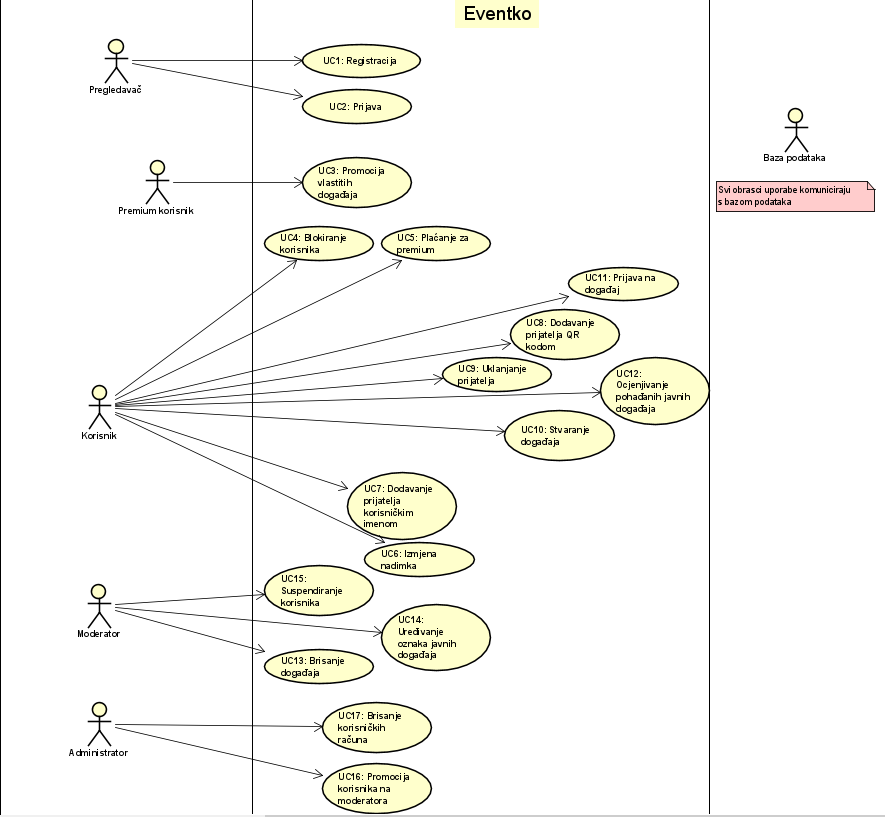
\includegraphics{slike/UseCase.jpg}
					
					
				\eject		
				
			\subsection{Sekvencijski dijagrami}
				
				\textbf{\textit{dio 1. revizije}}\\
				
			
				
				\noindent \textbf {Obrazac uporabe UC1 -Registracija}\\
				\noindent {Korisnik šalje zahtjev za prikaz Prijava stranice da bi mogao odabrati gumb za registraciju. Korisnik onda šalje zahtjev za prikaz Registracija stranice. Upisuje podatke potrebne za izradu računa koje Web aplikacija šalje bazi podataka koja radi profil. Baza vraća potvrdu nakon izrađenog profila i korisnik je vraćen na prikaz Prijava stranice.}
				
				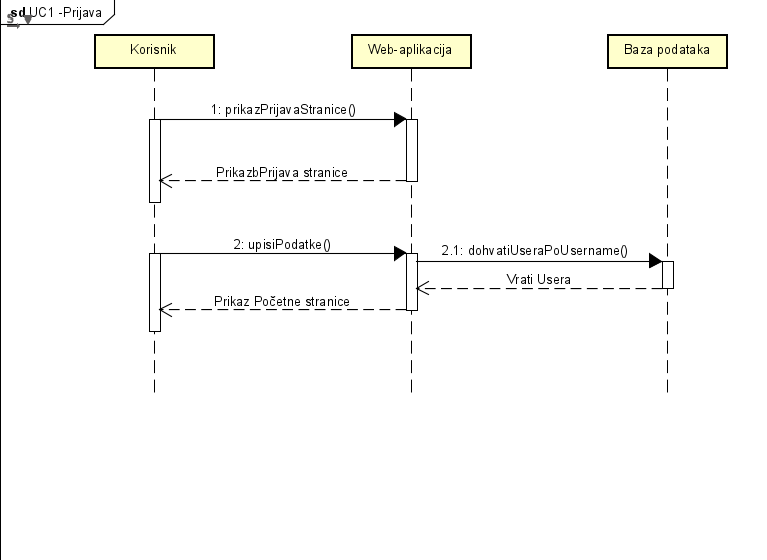
\includegraphics{slike/UC1 -Prijava}
				\eject
				
				\noindent \textbf {Obrazac uporabe UC1 -Registracija}\\
				\noindent {Korisnik šalje zahtjev za prikaz Prijava stranice nakon kojeg upisuje potrebne podatke za prijavu. Web aplikacija šalje podatke bazi podataka koja dohvaća korisnike i traži zadanog korisnika prema imenu profila. Baza podataka vraća profil korisnika nakon kojeg je korisniku prikazana Početna stranica }
				
				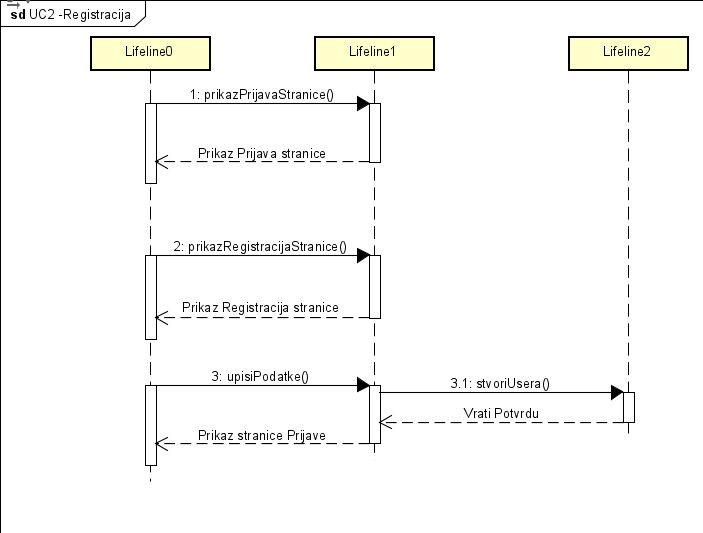
\includegraphics{slike/UC2 -Registracija.png}
				
				\eject
	
		\section{Ostali zahtjevi}
		
			\textbf{\textit{dio 1. revizije}}\\
		 
			 \textit{Nefunkcionalni zahtjevi i zahtjevi domene primjene dopunjuju funkcionalne zahtjeve. Oni opisuju \textbf{kako se sustav treba ponašati} i koja \textbf{ograničenja} treba poštivati (performanse, korisničko iskustvo, pouzdanost, standardi kvalitete, sigurnost...). Primjeri takvih zahtjeva u Vašem projektu mogu biti: podržani jezici korisničkog sučelja, vrijeme odziva, najveći mogući podržani broj korisnika, podržane web/mobilne platforme, razina zaštite (protokoli komunikacije, kriptiranje...)... Svaki takav zahtjev potrebno je navesti u jednoj ili dvije rečenice.}
			 \begin{packed_item}
			 \item  Sustav treba omogućiti rad više korisnika u stvarnom vremenu
			 \item Izvršavanje dijela programa u kojem se pristupa bazi podataka ne smije trajati duže od nekoliko sekundi
			 \item Sustav treba biti implementiran kao web aplikacija koristeći objektno-orijentirane jezike
			 \item Neispravno korištenje korisničkog sučelja ne smije narušiti funkcionalnost i rad sustava
			 \item Sustav treba biti jednostavan za korištenje, korisnici se moraju znati koristit sučeljem bez opširnih uputa
			 \item Nadogradnja sustava ne smije narušavati postojeće funkcionalnosti sustava
			 \item Veza s bazom podataka mora biti kvalitetno zaštićena, brza i otporna na vanjske greške
			 \end{packed_item}
	